\chapter{Introduction}
\label{sec:introduction}

Today, we use a number of computing devices interchangeably on a daily basis: a desktop workstation at the office,
a laptop computer on the move, a tablet in the living room and of course, always by our side, the smartphone.
In an increasingly cloudified and mobile world our expectation is to be able to do our work all the same,
regardless of the computing device we use, or where we are.

We start editing a text document in Google Docs on our desktop workstation at the office,
work on it a bit more on our laptop while travelling by train,
and proofread it later on the smartphone.
This device- and location-independent way of working has become the standard in recent years,
and users have started to expect it from their IT devices.

It's difficult to meet this expectation with the way electronic signatures are usually created today,
using certificates stored on on smartcards,
plugged into a laptop,
using a specialised card reader and accompanying software.
It's annoying and inconvenient having to carry around cables and adaptors, and a lot can go wrong:
a random operating system update breaking driver compatibility with the card reader, for example,
leaving us dead in the water.
If we want to make this easier on the user and to drive usage of electronic signatures and even make them mainstream,
we have to do better.

At the root of this inconvenience is the requirement that the user keep their private key physically with them,
stored in a manner making it difficult for anyone to steal it: on a smartcard.
Any IT professional knows full well this demand isn't made from users in order to annoy them but because it is
- more or less - the only practical \textit{and} secure way to have users store their private key.

So-called Remote Signing Services aim to eliminate the need for people to carry their private key with them,
and to locally create signatures,
in the hope for improved ease of use, and eventually, greater adoption of digitally signing documents.
However, allowing someone (the signing service, in this case) to be able to sign documents in place of the user introduces a number of serious security and confidentiality problems.


In this thesis, we analyse and address these problems,
and we implement the proposed solutions in a fully functional Remote Signing Service,
thereby showing that they work in the real world and not just on paper.

We will allow people to create electronic signatures,
no matter where they are, or what device they're using,
in a secure manner.
Building on our previous work of Project 2~\cite{projekt2}, we show how it is possible to securely integrate \gls{OIDC} authentication with remote digital signatures.
We expand upon this previous work and show how it is possible to have a remote signing service with the capability of signing on the users' behalf without the need for completely trusting that service.
Furthermore, we compare our solutions to those proposed by an industrial consortium led by Adobe Inc.,
and we show in which ways we believe our approach to be superior.

\subsection{Purpose of this document}\label{subsec:purpose-of-this-document}

In this document we will outline the objectives, scope and methodologies for our thesis as well as provide a project timeline.
The implementation will be documented separately.

\section{A cryptographic primer}\label{sec:a-cryptographic-primer}
In this section we well very briefly introduce the most important IT security and cryptography building blocks we use to make remote digital signing possible.
Readers with a basic knowledge of IT security topics such as hash functions, X.509, \gls{PKI} and \gls{DSA} can safely skip it.
The descriptions given are as brief as possible in order to introduce the topics, they're not meant to be complete nor excruciatingly precise.

\subsection{Hash Function}\label{subsec:hash-function}
A hash function in cryptography is an one-way function which is able to map data of arbitrary length to fixed-size values~\cite{hashing}.
One-way means that for a given hash value, it is infeasible to find the corresponding input data.
Ideally, the only way for someone to invert such a hash function is to do an exhaustive brute-force search.
This is called pre-image resistance.
Furthermore, a cryptographic hash function needs to fulfil the following properties:
\begin{enumerate}
    \item For a given input value, it must always produce the same hash value (it must be deterministic)
    \item It must be infeasible to find to different input values that produce the same hash value (this is called collision resistance)
    \item For a given input value, it must be infeasible to find another input value that produces the same hash value (second pre-image resistance)
    \item A minimal change in the input value must result in a completely different output value (avalanche effect)
\end{enumerate}

Hash functions fulfilling these properties are fundamental to our work (and to much of cryptography in general).
Without them we would be completely powerless.
An example for such a hash function is \gls{SHA-2}~\cite{sha2patent}.

\subsection{Asymmetric cryptography}\label{subsec:asymmetric-cryptography}
Asymmetric cryptography, sometimes called public-key cryptography, is a type of encryption which uses pairs of keys.
This is in contrast to symmetric encryption which uses only one key (for example, a passphrase encrypting a file).

With symmetric encryption the passphrase must me known both to encrypt and to decrypt the message,
but with public-key cryptography, the public key can be used to encrypt a message and the private key to decrypt it.

This might sound simple on the surface but opens up a world of possibilities.
Only the private key has to be kept secret, the public key can be freely published~\cite{stallings}.

The classical example for such an encryption system is the \gls{RSA} scheme~\cite{rsa}.

For a simplified example how public-key-based encrypted communication between two parties could work,~\footnote{
We're well aware of the major security problems in this example,
like the fact that both the key exchange and the message exchange happen unauthenticated and without integrity protection,
but we intentionally chose to keep the example as simple as possible in order to keep it easily comprehensible by a wide audience.
}
see figure~\ref{fig:simplepubkeycomm}.

\begin{figure}[H]
    \centering
    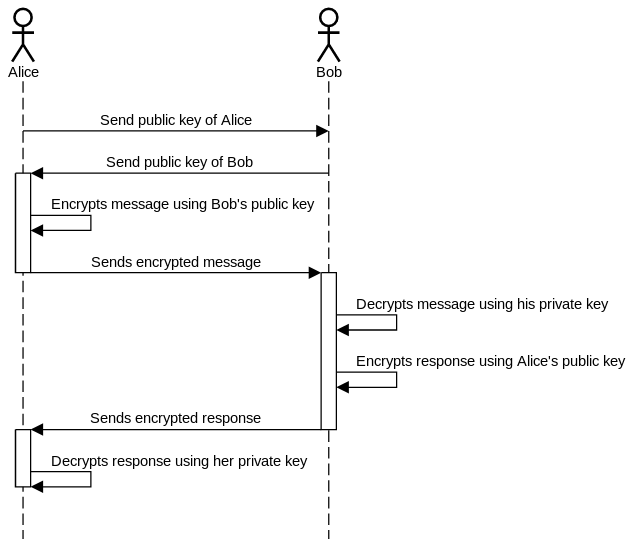
\includegraphics[width=0.75\textwidth]{images/simplistic_pubkey_communication.png}
    \caption{Simplified example of two Actors, Alice and Bob, exchanging encrypted messages using public-key cryptography}
    \label{fig:simplepubkeycomm}
\end{figure}


\subsection{Digital Signatures}\label{subsec:digital-signatures}
Having briefly explained Hash Functions in~\ref{subsec:hash-function} and Asymmetric Encryption in~\ref{subsec:asymmetric-cryptography} we can now move on to introducing digital signatures.
A digital signature is a way for verifying the integrity and authenticity of a message, that is,
to know who signed the message and to guarantee that it wasn't tampered with since being signed~\cite{digitalsignature}.

In order to create a digital signature, perform the following steps:
\begin{enumerate}
    \item We take our message and run it through a cryptographic hash function, thus obtaining the hash value.
    \item Then, we encrypt the hash value using our private key.
    \item Then we transmit the message and the encrypted hash value to the recipient.
\end{enumerate}

In order to verify the authenticity and integrity of the message, the recipient performs the following steps:
\begin{enumerate}
    \item They run the message through the same cryptographic hash function we did and obtain its hash value.
    \item They decrypt the encrypted hash value we sent them using our public key and compare it to the one they obtained themselves.
    \item If the values match, the recipient can be confident that a) the message wasn't tampered with and b) we authored and signed it.
\end{enumerate}

\subsection{Public-Key Infrastructure and Certificate Authorities}\label{subsec:public-key-infrastructure-and-certificate-authorities}
Asymmetric cryptography as described in~\ref{subsec:asymmetric-cryptography} looks like the perfect solution for private communication of any kind,
but unfortunately it presents us with a big challenge: key distribution.

TODO explain public key distribution problem and X.509 CAs

\subsection{Timestamps}\label{subsec:timestamps}
TODO explain timestamping services

